\chapter{Controlling program flow}
\label{chap:flow}
Non-recursive functions encapsulates code and allows for some control of flow, that is, if there is a piece of code, which we need to to have executed many times, then we can encapsulate it in the body of a function, and then call the function several times. In this chapter, we will look at more general control of flow via loops, conditional execution, and recursion, and therefore we look at further extension of the \lstinline[language=ebnf]!expr! rule,
\begin{lstlisting}[language=ebnf]
pat = const | ...
guard = "when" expr
rule = pat [guard] -> expr
rules = "|" rule | "|" rule rules (* first "|'' is optional' *)
expr = ... 
  | "for" pat "in" expr "do" expr ["done"] (* for expression *)
  | "for" var "=" expr "to" expr "do" expr ["done"] (* simple for expression *)
  | "while" expr "do" expr ["done"] (* while expression *)
  | "if" expr "then" expr {"elif" expr "then" expr} ["else" expr (*  conditional expression *)]
  | "match" expr "with" rules (* match expression *)
  | "function" rules (* matching function expression *)
  | "let" rec functionOrValueDefns (* recursive definition *)
  | ...
\end{lstlisting}

\section{For and while loops}
Many programming constructs need to be repeated. The most basic example is counting, e.g., from 1 to 10 with a \idx{\keyword{for}}-loop,\jon{Is it clear enough that the body of the loop is repeated?}
%
\fso{count}{Counting from 1 to 10 using a \keyword{for}-loop.}
%
As this interactive script demonstrates, the identifier \lstinline!i! takes all the values between 1 and 10, but in spite of its changing state, it is not mutable. Note also that the return value of the \keyword{for} expression is \lexeme{()} like the \lstinline!printf! functions. The \keyword{for} and \keyword{while} loops follow the syntax,
\begin{lstlisting}[language=ebnf]
pat = const | ...
expr = ... 
  | "for" pat "in" expr "do" expr ["done"] (* for expression *)
  | "for" var "=" expr "to" expr "do" expr ["done"] (* simple for expression *)
  | "while" expr "do" expr ["done"] (* while expression *)
 | ...
\end{lstlisting}
Using lightweight syntax the script block between the \idx{\keyword{do}} and \idx{\keyword{done}} keywords may be replaced by a newline and indentation, e.g.,
%
\fs{countLightweight}{Counting from 1 to 10 using a \keyword{for}-loop.}
%
A more complicated example is,
\begin{problem}
  Write a program that prints the $n$'th Fibonacci number.
\end{problem}
The Fibonacci numbers is the series of numbers $1,1,2,3,5,8,13\dots$, where the $\text{fib}(n) = \text{fib}(n-1)+\text{fib}(n-2)$, and they are related to Golden spirals shown in Figure~\ref{fig:goldenSpiral}.
\begin{figure}
  \centering
  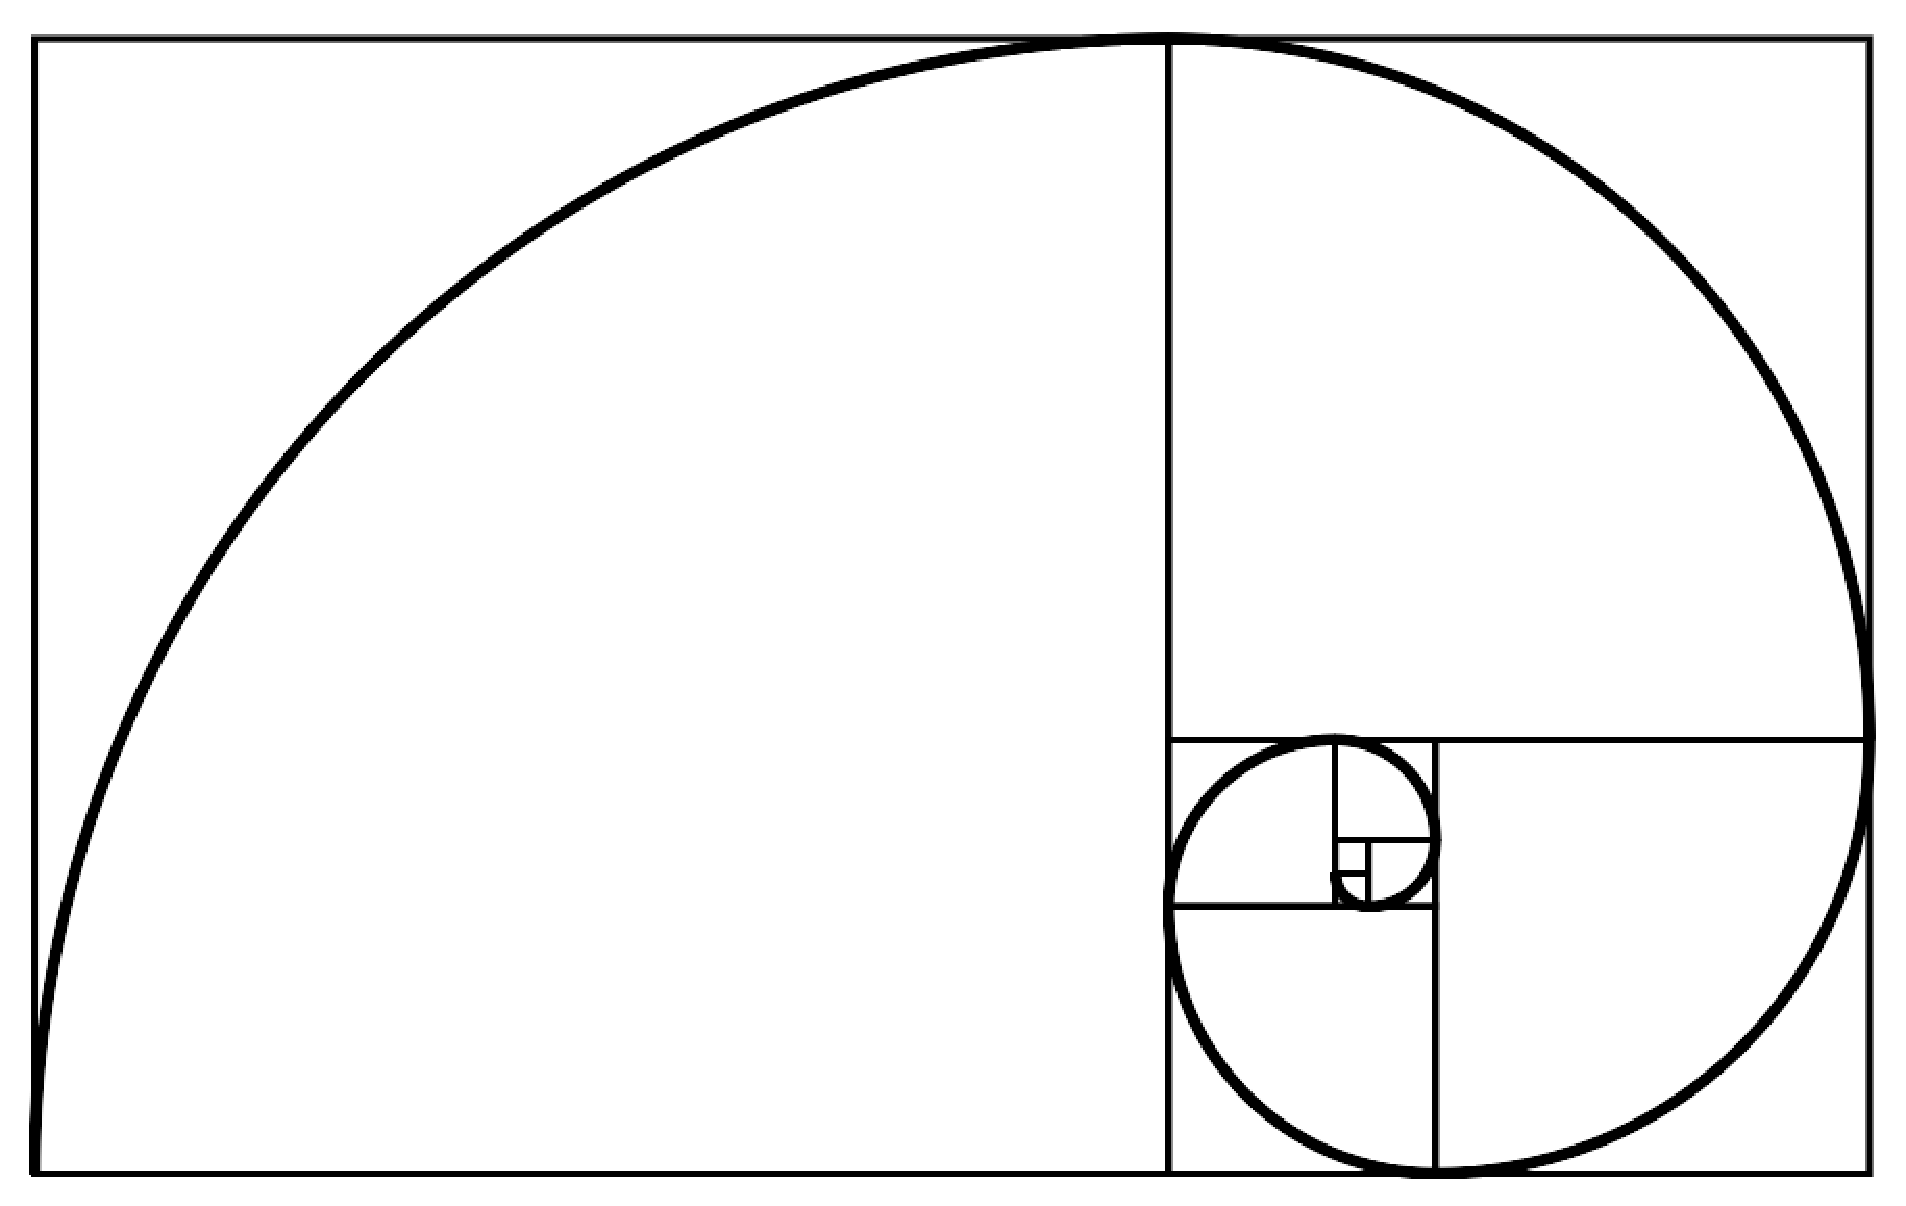
\includegraphics[width=0.45\linewidth]{Fibonacci_spiral_34}
  \caption{The Fibonacci spiral is an approximation of the golden spiral. Each square has side lengths of successive Fibonacci numbers, and the curve in each square is the circular arc with radius of the square it is drawn in. Figure by Dicklyon \url{https://commons.wikimedia.org/w/index.php?curid=3730979}}
  \label{fig:goldenSpiral}
\end{figure}
We could solve this problem with a \keyword{for}-loop as follows,
%
\fs{fibFor}{The $n$'th Fibonacci number as the sum of the previous 2 numbers, which are sequentially updated from 3 to $n$.}
%
The basic idea of the solution is that if we are given the $(n-1)$'th and $(n-2)$'th numbers, then the $n$'th number is trivial to compute. And assume that $\text{fib}(1)$ and $\text{fib}(2)$ are given, then it is trivial to calculate the $\text{fib}(3)$. Now we have the first 3 numbers, so we disregard $\text{fib}(1)$ and calculate $\text{fib}(4)$ from $\text{fib}(2)$ and $\text{fib}(3)$, and this process continues until we have reached the desired $\text{fib}(n)$

For the alternative \keyword{for}-loop, consider the problem,
\begin{problem}
  Write a program that identifies prime factors of a given integer $n$.
\end{problem}
Prime numbers are integers divisible only be 1 and themselves with zero remainder. Let's assume that we already have identified a list of primes from 2 to $n$, then we could write a program that checks the remainder as follows,
%
\fs{primeCheck}{Checking whether a given number has remainder zero after division by some low prime numbers.}
%
In this example, the variable \lstinline!i! runs through the elements of a list, which will be discussed in further detail in Chapter~\ref{chap:lists}.

The \idx{\keyword{while}}-loop is simpler than the \keyword{for}-loop and does not contain a builtin counter structure. Hence, if we are to repeat the count-to-10 program from Listing~\ref{count} example, it would look somewhat like,
%
\fs{countWhile}{Count to 10 with a counter variable.}
%
In this case, the \keyword{for}-loop is to be preferred, since more lines of code typically means more chances of making a mistake. But the \keyword{while}-loop allows for other logical structures. E.g., lets find the biggest Fibonacci number less than 100,
%
\fs{fibWhile}{Search for the largest Fibonacci number less than a specified number.}
%
Thus, \keyword{while}-loops are most often used, when the number of iteration cannot easily be decided, when entering the loop.

Both \keyword{for}- and \keyword{while}-loops are often associated with variables, i.e., values that change while looping. If one mistakenly used values and rebinding, then the result would in most cases be of little use, e.g.,
%
\fs{forScopeError}{Lexical scope error. While rebinding is valid F\# syntax, has little effect due to lexical scope.}
%
I.e., the \keyword{let} expression rebinds \lstinline!a! every iteration of the loop, but the value on the right-hand-side is taken lexically from above, where \lstinline!a! has the value 1, so every time the result is the value 2.

\section{Conditional expressions}
Consider the task,
\begin{problem}
  Write a function that given $n$ writes the sentence, ``I have n apple(s)'', where the plural 's' is added appropriately.
\end{problem}
For this we need to test on $n$'s size, and one option is to use conditional expressions like,
%
\fse{conditional}{Using conditional expression to generate different strings.}
%
The grammar for conditional expressions is,
\begin{lstlisting}[language=ebnf]
expr = ... 
  | "if" expr "then" expr {"elif " expr "then" expr} ["else" expr] (*  conditional expression *)
  | ...
\end{lstlisting}
where the \lstinline[language=ebnf]!expr! following \idx{\keyword{if}} and \idx{\keyword{elif}} are \idx{conditions}, i.e., expressions that evaluate to a boolean value. The \lstinline[language=ebnf]!expr! following \idx{\keyword{then}} and \idx{\keyword{else}} are called \idx{branches}, and all branches must have same type. The result of the conditional expression is the first branch, for which its condition was true. The lightweight syntax allows for the visually more simple expression of scope by use of indentation
%
\fse{conditionalLightweight}{Lightweight syntax allows for making blocks of code by indentation in order to make code more for easy to read.}
%
Note that both \keyword{elif} and \keyword{else} branches are optional, which may cause problems, e.g., both \lstinline!let a = if true then 3! and \lstinline!let a = if true then 3 elif false then 4!  will be invalid, since F\# is not smart enough to realize that the type of the expression is uniquely determined. Instead F\# looks for the \keyword{else} to ensure all cases have been covered, and that \lstinline!a! always will be given a unique value of the same type regardless of the branches taken in the conditional statement, hence, \lstinline!let a = if true then 3 else 4!  is the only valid expression of the 3. However, the omitted branches are assumed to return \lexeme{()}, and thus it is fine to say \lstinline!let a = if true then ()! and \lstinline!if true then printfn "hej"!

\subsection{Programming intermezzo}
Using loops and conditional expressions we are now able to solve the following problem
\begin{problem}
  Given an integer on decimal form, write its equivalent value on binary form
\end{problem}
To solve this problem, consider odd numbers: They all have the property, that the least significant bit is 1, e.g., $1_2 = 1, 101_2 = 5, 110_2 = 6$, and that division by 2 is equal to right-shifting by 1, e.g., $1_2/2 = 0.1_2 = 0.5, 101_2/2 = 10.1_2 = 2.5, 110_2/2 = 11_2 = 3$. Thus by integer division by 2 and checking the remainder, we may sequentially read off the least significant bit. This leads to the following algorithm,
%
\fs{dec2bin}{Using integer division and remainder to convert any positive integer to binary form.}
%


% since in, e.g., \keyword{let} expressions, F\# requires all cases to be covered, 

% A basic flow control mechanism used both for functional and imperative programming is the \texttt{if-then-else} construction, e.g.,
% \fs{flowIfThen}{}
% I.e., if and only if the value of the argument is postive, then it will be printed on screen. More common is to include the \texttt{else} 
% \fs{flowIfThenElse}{}
% A common construction is a nested list of \texttt{if-then-else},
% \fs{flowIfThenElseNested}{}
% where the integers 0--2 are converted to characters, and integers outside this domain is converted to the nearest equivalent number. This construction is so common that a short-hand notation exists, and we may equivalently have written,
% \fs{flowIfThenElseNestedShort}{}

\section{Pattern matching}
Conditional expressions are so common that a short-hand notation called \idx{pattern matching} is available in F\#. For the 
Consider the task,
\begin{problem}
  Write a function that given $n$ writes the sentence, ``I have n apple(s)'', where the plural 's' is added appropriately.
\end{problem}
For this we need to test on $n$'s size, and one option is to use conditional expressions like,
%
\fs{matchWith}{Using the \keyword{match}-keyword{with} programming construct to vary calculation based on the input value.}
%
Here the \idx{\keyword{match}}-\idx{\keyword{with}} keywords starts a sequence of conditions separated by the \lexeme{|} lexeme, where the default operator is the \lexeme{=} comparison operator, but where others can be used with the \idx{\keyword{when}}. The syntax of \keyword{match} expressions is,
\begin{lstlisting}[language=ebnf]
pat = const | "_" | ...
guard = "when" expr
rule = pat [guard] -> expr
rules = "|" rule | "|" rule rules (* first "|'' is optional' *)
expr = ... 
  | "match" expr "with" rules (* match expression *)
  | "function" rules (* matching function expression *)
  | ...
\end{lstlisting}
As for conditional expressions, the rules are treated sequentially from first to last, and the expression following the first rule with a true condition is the the result of the entire expression. The rules are versatile in their possible expression, e.g., the line \lstinline!| 1 -> "I have no apples"! is equivalent to \lstinline!elif n < 1 then "I have no apples"|, and the \lstinline!| \_ -> "I have " + (string n) + " apples"!, matches the \lstinline!else "I have " + (string n) + " apples"!, since the \lexeme{_} lexeme is a wildcard pattern matching anything. Finally, the first rule is a guarded rule indicated by the \keyword{when} keyword, \lstinline!i when i < 0 -> "I owe " + (string -i) + " apples"!. It uses the optional disregard of the \lexeme{|} lexeme and is equivalent to \lstinline!if n < 0 then "I owe " + (string -n) + " apples"!. Guarded rules can be any rules, and here we used the identifier \lstinline!i! meaning \lstinline!let i = n in if i < 0 then ...!, i.e., \lstinline!n! is renamed. One way to think of guarded expressions is that \lstinline!i when i < 0! is a set, and the condition is on \lstinline!n! being part of the set or not. 

Using lightweight syntax, the rules may be put on separate lines but must start in the column, where the \keyword{match} starts or greater.\jon{Spec-4.0 weirdness: Offside rule for match is different for function.} Match with can only take one identifier, but this can be tuples for matching with combinations of identifiers, see Chapter~\ref{chap:lists} for more on tuples. A \keyword{match} expression is general but is most often seen as the initial part of a function definition. This is so common, that F\# has a special syntax integrating function definitions and match with expressions using the \idx{\keyword{function}} keyword,
%
\fs{functionKeyword}{Function definition and \keyword{match} expressions are integrated using the \keyword{function} keyword. Compare with Listing~\ref{matchWith}}
%
Comparing with Listing~\ref{matchWith} notice that the function definition does not explicitly name an argument but assumes one, following the \keyword{function} follows immediately the rules, and the wildcard pattern \lexeme{_} is replaced with an identifier without any guards, which thus matches everything. Replacing the wildcard pattern with a name has the advantage that this name can be used locally in the expression belonging to this rule, i.e., it acts as a \lstinline!let n = ! on the implicit argument of the function. Implicit arguments makes the code hard to read and, thus \advice{the use of function definitions with the keyword \keyword{function} should be avoided.}

\section{Recursive functions}
Recursion is a central concept in F\#. A \idx{recursive function} is a function, which calls itself. From a compiler point of view, this is challenging, since the function is used before the compiler has completed its analysis. However, this there is a technical solution for, and we will just concern ourselves with the logics of using recursion for programming. An example of a recursive function that counts from 1 to 10 similarly to Listing~\ref{count} is,\jon{A drawing showing the stack for the example would be good.}
%
\fs{countRecursive}{Counting to 10 using recursion.}
%
Here the \lstinline!prt! calls itself repeatedly, such that the first call is \lstinline!prt 1 10!, which calls \lstinline!prt 2 10!, and so on until the last call \lstinline!prt 10 10!. Calling \lstinline!prt 11 10! would not result in recursive calls, since when \lstinline!a! is higher than \lstinline!10! then the \idx{stopping criterium} is met and a newline is printed. For values of \lstinline!a! smaller than or equal \lstinline!b! then the recursive branch is executed. Since \lstinline!prt! calls itself as the last all but the stopping condition, then this is a \idx{tail-recursive} function. Most compilers achieve high efficiency in terms of speed and memory, so \advice{prefer tail-recursion whenever possible.}
\begin{lstlisting}[language=ebnf]
functionOrValueDefnList = 
  functionOrValueDefn 
  | functionOrValueDefn "and" functionOrValueDefnList
expr = ... 
  | "let" rec functionOrValueDefnList (* recursive definition *)
  | ...
\end{lstlisting}
Using recursion to calculate the Fibonacci number as Listing~\ref{fibFor}.
%
\fs{fibRecursive}{The $n$'th Fibonacci number using recursive.}
%
Here we used the fact that including $\text{fib}(0)=0$ in the Fibonacci series also produces it using the rule $\text{fib}(n)=\text{fib}(n-2)+\text{fib}(n-1),\; n\geq 0$, which allowed us to define a function that is well defined for the complete set of integers. I.e., a negative argument returns 0. This is a general advice: \advice{make functions that fails gracefully.} The recursive definition allows for recursive value definitions and defining several values and functions in one expression. Recursive values is particularly useful for defining infinite sequences, see Section~\ref{sec:sequences}.

% Functions may be declared using pattern matching, which is a flexible method for declaring output depending on conditions on the input value. The most common pattern matching method is by use of the \texttt{match with} syntax,
% \fs{functionDeclarationMatchWith}{}

% A short-hand only for functions of 1 parameter is the \texttt{function} syntax,
% \fs{functionDeclarationFunction}{}
% Note that the name given in the match, here \texttt{n}, is not used in the first line, and is arbitrary at the line of pattern matchin, and may even be different on each line. For these reasons is this syntax discouraged.

%%% Local Variables:
%%% TeX-master: "fsharpNotes"
%%% End:
